\documentclass[xcolor=dvipsnames]{beamer} 

\usepackage[T1]{fontenc}
\usepackage[utf8]{inputenc} %caractères spéciaux
\usepackage[french]{babel} %français
\usepackage{graphicx}
\usepackage[absolute]{textpos}

\usepackage{amsmath}
\usepackage{amsfonts}
\usepackage{amssymb}

\usepackage{xspace} %symboles extensifs

\setbeamercovered{dynamic} %prevent losing position when using dynamic

\usetheme{Darmstadt}
\usecolortheme{seahorse}


\newcommand{\p}[2]{\ensuremath{\frac{\partial {#1}}{\partial {#2}}}}
\newcommand{\tot}[2]{\ensuremath{\frac{d {#1}}{d {#2}}}}

\newcommand{\vs}{\ensuremath{\mathbf{v}^s}}

\newcommand{\bfr}{\ensuremath{\mathbf{r}}}

\newcommand{\om}[1]{\ensuremath{ \mathcal{O} \left( {#1} \right) }}

\newcommand{\ttt}[1]{ \texttt{#1} }

\newcommand{\hphi}{\ensuremath{\hat{\phi}}}
\newcommand{\z}{\ensuremath{\zeta}}
\newcommand{\x}{\ensuremath{\xi}}
\newcommand{\zperp}{\ensuremath{\zeta^\perp}}
\newcommand{\lam}{\ensuremath{\lambda}}

\title[Étude du point de Lifshitz par le groupe de renormalisation.]{Étude du point de Lifshitz par le groupe de renormalisation.}
\date{Stage du 13 janvier au 7 mars 2014 au \\ 
Laboratoire de physique théorique de la matière condensée (LPTMC) \\ 
\small{UMPC}}
\author{Nicolas Macé \\
\textbf{Responsable de stage :} Dominique Mouhanna}

\begin{document}

\begin{frame}
\begin{titlepage}
\end{titlepage}
\end{frame}


\section{Le modèle de Lishitz}

\section{Le groupe de renormalisation non perturbatif}
\subsection{L'idée de la renormalisation}
\begin{frame}

\only<1>{
\begin{figure}[htp]
\centering

\includegraphics[scale=0.35]{img/renorm_step0.pdf}
\label{}
\end{figure}
\[H[\phi(x_i)]\]
\[\phantom{\tilde{\phi}_B = \frac{1}{Sa} \sum_{i \in B} \phi_i}\]
}

\only<2>{
\begin{figure}[htp]
\centering
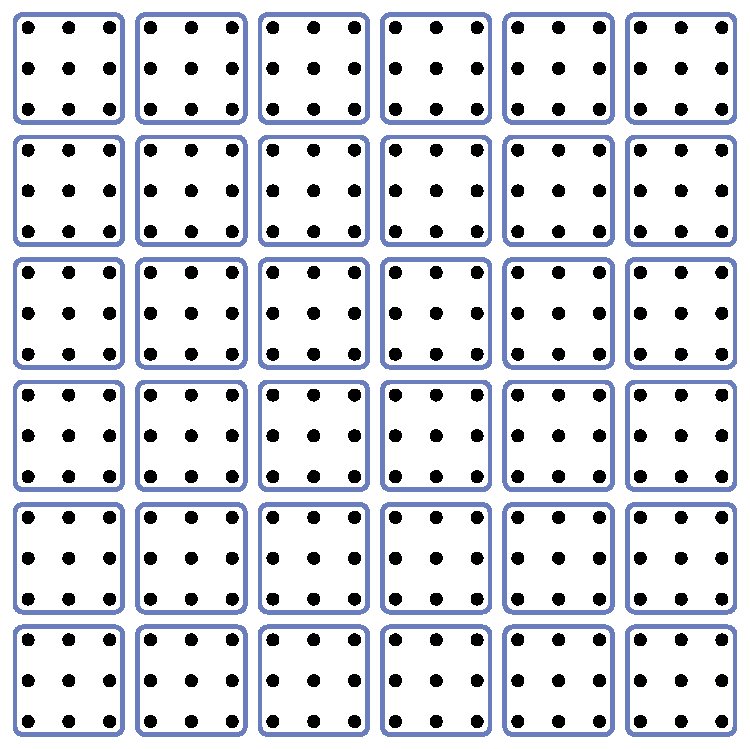
\includegraphics[scale=0.35]{img/renorm_step1.pdf}
\label{}
\end{figure}
\[H[\phi(x_i)]\]
\[\tilde{\phi}(x_b) = \frac{1}{Sa} \sum_{i \in b} \phi(x_i)\]
}

\only<3>{
\begin{figure}[htp]
\centering
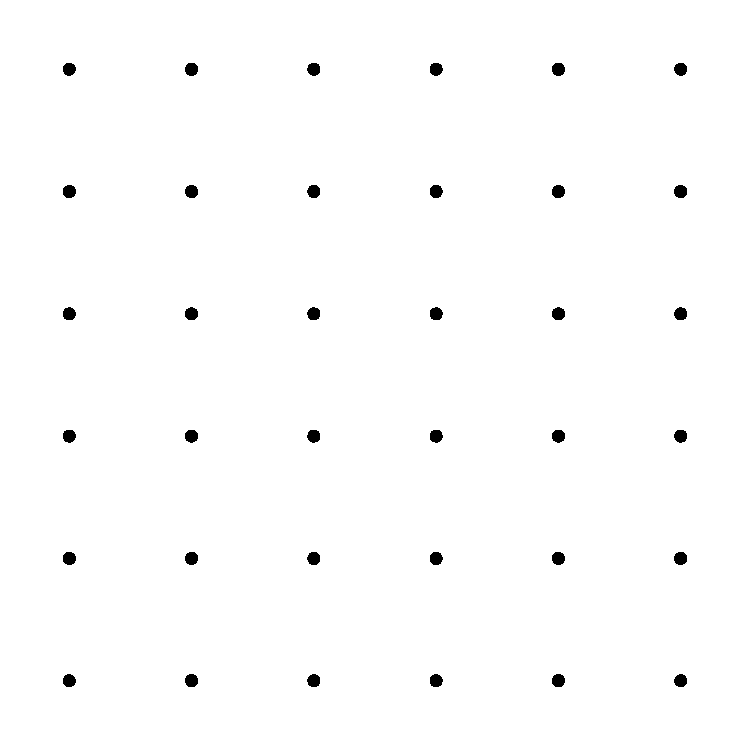
\includegraphics[scale=0.35]{img/renorm_step2.pdf}
\label{}
\end{figure}
\[H[\phi(x_i)] \rightarrow \tilde{H}[\tilde{\phi}(x_b)]\]
\[\phantom{\tilde{\phi}_b = \frac{1}{Sa} \sum_{i \in b} \phi_i}\]
}

\only<4>{
\begin{figure}[htp]
\centering

\includegraphics[scale=0.35]{img/renorm_step3.pdf}
\label{}
\end{figure}
\[
 \left.\begin{aligned}
        x' = x/S \\
        \phi' = S^\Delta \phi
       \end{aligned}
 \right\}
  \rightarrow H_S[\phi'(x'_i)]
\]
Comparer $H$ et $H_S$ $\rightarrow$ renormalisation des constantes de couplage.
}
  
\end{frame}

\subsection{Application au modèle de Lifshitz en champ moyen}
\begin{frame}

\begin{columns}

\begin{column}{6cm}
\[
	\p{}{t} \phi + \nabla \cdot ( \mathbf{u} \phi )  - q \p{}{z} \phi( 1 - \phi) = 0
\]
\end{column}

\begin{column}{6cm}
\[
 \text{Fraction volumique } \phi = \frac{d\tau^s}{d\tau^l + d\tau^s} 
\]
\end{column}

\end{columns}

\end{frame}

\subsection{Le groupe de normalisation non perturbatif}

\section{Le point critique de Lifshitz : méthodes et résultats}
\subsection{L'Anzatz pour l'action effective du modèle}
\begin{frame}

\begin{columns}

\begin{column}{6cm}

\end{column}

\begin{column}{6cm}

\end{column}

\end{columns}

~ \\
~ \\
~ \\
\begin{centering}
couplage ségrégation et convection : canalisation de l'écoulement 
\end{centering}

\begin{centering}
$\rightarrow$ analyse du phénomène \textit{pendant} l'écoulement
\end{centering}
\end{frame}

\subsection{Flots de renormalisation}
\begin{frame}


\end{frame}

\subsection{Équations de point fixe}
\begin{frame}

\begin{columns}

\begin{column}{6cm}

\only<1>{
}

\only<2-3>{
}\par

\end{column}

\begin{column}{6cm}

\only<1-2>{
}

\only<3>
{

\[
		\begin{pmatrix}
	u(x, y, z)\\
	v(x, y, z)\\
\end{pmatrix}
=
f \left( \frac{z}{h} \right)
\begin{pmatrix}
	\bar u(x, y) \\
	\bar v(x, y) \\
\end{pmatrix}
\]

\[
	\p{}{t} \phi + \nabla \cdot ( \mathbf{u} \phi )  - q \p{}{z} \phi( 1 - \phi) = 0
\]

}

\end{column}

\end{columns}

\end{frame}

\subsection{Le potentiel au point de Lifshitz}

\subsection{Les exposants critiques}

\section{Conclusion}
\begin{frame}

\begin{itemize}
\item modélisation d'un phénomène mal compris : la ségrégation
\item relations entre physique, mathématiques et analyse numérique 
\item un domaine de la physique nouveau et en plein essor
\end{itemize}

\end{frame}

\end{document}